В ходе реализации синтезируемых компонентов модуля Remap активно использовалось тестирование с помощью симуляции. Оно осуществлялось с помощью специализированного программного обеспечения Mentor QuestaSim, предназначенное для моделирования и отладки микросхем ПЛИС. Симуляционное окружение разработано, как и синтезируемые модули, на языке VHDL и обеспечивает поступление данных на входной интерфейс тестируемого модуля. Так, на рисунке \ref{fig:sim_input} приведён фрагмент симуляции, на котором показан пример данных внутри внутри  входного интерфейса. Можно увидеть, что как и в реальной системе, в каждый модуль Remap поступает 22 канала со значениями АЦП, причем для каждого BCID передаётся по 8 величин в канале. Все сигналы входного сигнала синхронны с тактовой частотой $f_{feb}$.\par
\begin{figure}[ht]
    \centering
    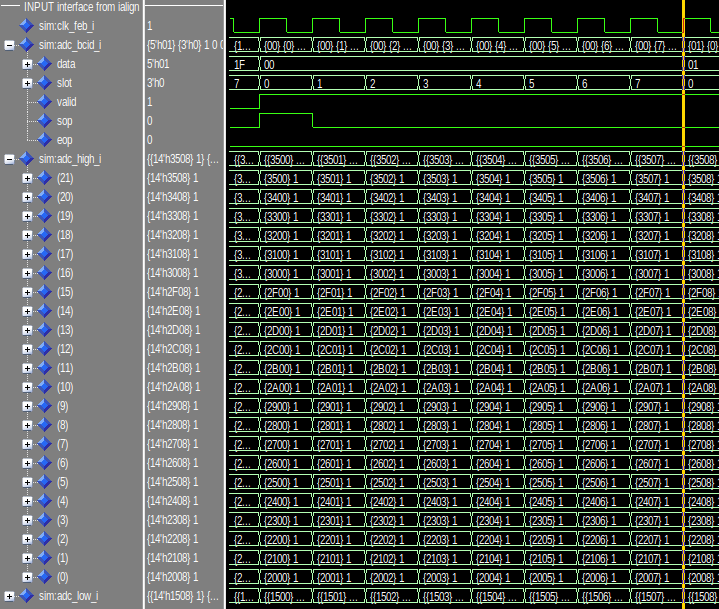
\includegraphics[width=\linewidth]{sim_input.png}
    \caption{Фрагмент поступающих в модуль Remap входных данных в симуляции}
    \label{fig:sim_input}
\end{figure}\par
В рассматриваемом примере модуль предназначен для работы в варианте сигнального процессора LASP с установленной медленной опцией. В качестве конфигурации производится установка параметров для первых двух выходных каналов Remap компонента. На рисунке \ref{fig:sim_sctrl} отображено, как это осуществляется через интерфейс медленного контроля. На волновой диаграмме отчетливо видно, как значения поступают в установленном формате по протоколу AVMM, после чего лишние биты отсекаются, а сами конфигурационные данных переходят в соответствующие им тактовые домены. В соответствии с настройкой, первый выходной канал должен выдавать данные из первых восьми входных каналов в обратной последовательности, а второй по четыре значения из каналов с номерами 20 и 21 в чередующейся последовательности.\par
\begin{figure}[ht]
    \centering
    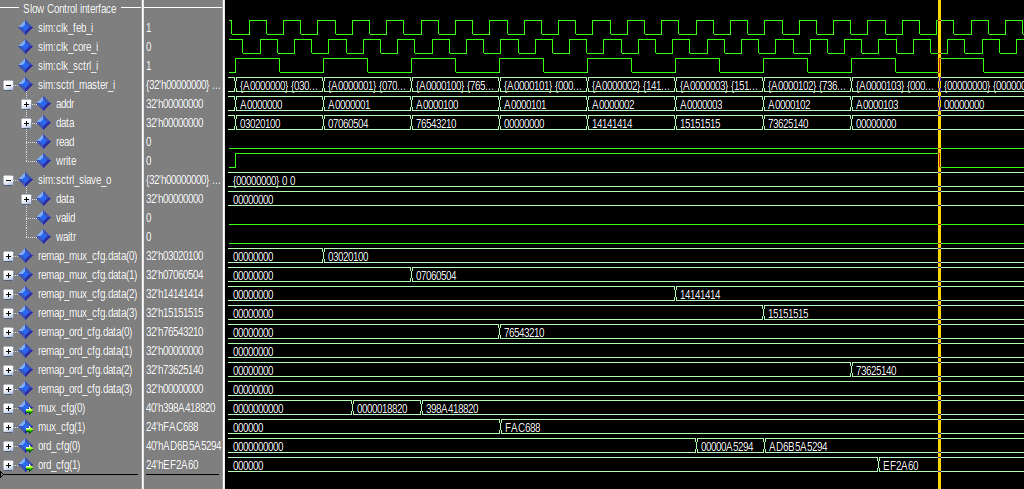
\includegraphics[width=\linewidth]{sim_sctrl.png}
    \caption{Пример записи конфигурации модуля Remap в симуляции}
    \label{fig:sim_sctrl}
\end{figure}\par
На рисунке \ref{fig:sim_output} изображен выходной интерфейс модуля конфигурируемой перестановки. Поскольку система предназначена для работы в медленной опции сигнального процессора LASP, выходной интерфейс состоит из 16 каналов, в котором данные передаются синхронно частоте $f_{core}$, равной 320 МГц. На нём можно отследить корректность работы компонента, работающего в соответствии с вышеописанными настройками. \par
\begin{figure}[ht]
    \centering
    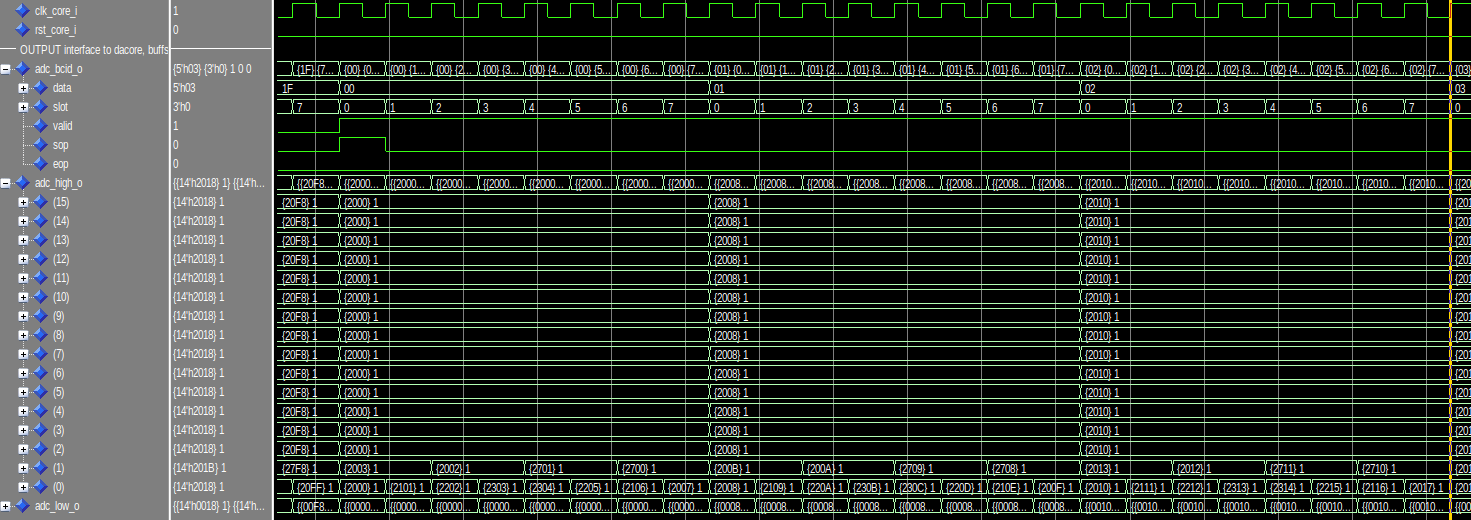
\includegraphics[width=\linewidth]{sim_output.png}
    \caption{Фрагмент выходящих из модуля Remap данных в симуляции}
    \label{fig:sim_output}
\end{figure}\par
